%% LyX 2.3.6.1 created this file.  For more info, see http://www.lyx.org/.
%% Do not edit unless you really know what you are doing.
\documentclass[english]{article}
\usepackage[T1]{fontenc}
\usepackage[latin9]{inputenc}
\usepackage{geometry}
\geometry{verbose,tmargin=2.5cm,bmargin=2.5cm,lmargin=2.5cm,rmargin=2.5cm}
\usepackage{textcomp}
\usepackage{graphicx}

\makeatletter

%%%%%%%%%%%%%%%%%%%%%%%%%%%%%% LyX specific LaTeX commands.
%% Because html converters don't know tabularnewline
\providecommand{\tabularnewline}{\\}

\makeatother

\usepackage{babel}
\begin{document}
{[}SPLIT\_HERE{]}
\begin{enumerate}
\item \textbf{{[}PJC/PRELIM/9597/2016/P1/Q1{]} }

Four stories are given in four data files: \texttt{AIRCON.txt}, \texttt{BLIND.txt},
\texttt{COMP.txt}, \texttt{EMPEROR.txt}. The task is to find the frequency
of alphabets used in the stories. 

\subsection*{Task 1.1 }

Count the alphabets in each story and display the frequency of each
alphabet in a table form. Do not distinguish between upper and lower
cases. Do not count non-alphabets. Frequency should be displayed in
descending order. Display alphabets with same frequency in ascending
order. 

Sample output: 
\noindent \begin{center}
\begin{tabular}{lll}
\texttt{Alphabet} & \texttt{Frequency} & \tabularnewline
\texttt{e} & \texttt{20} & \tabularnewline
\texttt{t} & \texttt{14} & \tabularnewline
\cline{3-3} 
\texttt{a} & \multicolumn{1}{l|}{\texttt{12}} & \multicolumn{1}{l|}{\texttt{a} and \texttt{i} have same frequency of 12,}\tabularnewline
\texttt{i} & \multicolumn{1}{l|}{\texttt{12}} & \multicolumn{1}{l|}{display \texttt{a} before \texttt{i}, since \texttt{a} comes before
\texttt{i}}\tabularnewline
\cline{3-3} 
\texttt{o} & \texttt{10} & \tabularnewline
\texttt{u} & \texttt{6} & \tabularnewline
\cline{3-3} 
\texttt{g} & \multicolumn{1}{l|}{\texttt{3}} & \multicolumn{1}{l|}{\texttt{g} and \texttt{j} have same frequency of 12,}\tabularnewline
\texttt{j} & \multicolumn{1}{l|}{\texttt{3}} & \multicolumn{1}{l|}{display \texttt{g} before \texttt{j,} since \texttt{g} comes before
\texttt{j}}\tabularnewline
\cline{3-3} 
\texttt{z} & \texttt{1} & \tabularnewline
\end{tabular}
\par\end{center}

\subsection*{Evidence 1: }

Your program code for task 1.1.\hfill{} {[}9{]}

\subsection*{Evidence 2: }

Screenshot of running \texttt{AIRCON.txt} data file.\hfill{} {[}1{]}

\subsection*{Task 1.2 }

Amend your program code to display alphabets and frequencies in all
four files in a table form, with alphabets in first column and frequencies
of alphabets in subsequent columns. Display in alphabetical order
as shown in following sample output: 
\noindent \begin{center}
\begin{tabular}{|l|l|l|l|l|}
\hline 
\texttt{Alphabet} & \texttt{AIRCON.txt} & \texttt{BLIND.txt} & \texttt{COMP.txt} & \texttt{EMPEROR.txt}\tabularnewline
\hline 
\texttt{a} & \texttt{115} & \texttt{471} & \texttt{604} & \texttt{490}\tabularnewline
\hline 
\texttt{b} & \texttt{25} & \texttt{87} & \texttt{111} & \texttt{56}\tabularnewline
\hline 
\texttt{c} & \texttt{46} & \texttt{117} & \texttt{230} & \texttt{107}\tabularnewline
\hline 
\texttt{$\vdots$} & \texttt{$\vdots$} & \texttt{$\vdots$} & \texttt{$\vdots$} & \texttt{$\vdots$}\tabularnewline
\hline 
\texttt{$\vdots$} & \texttt{$\vdots$} & \texttt{$\vdots$} & \texttt{$\vdots$} & \texttt{$\vdots$}\tabularnewline
\hline 
\texttt{x} & \texttt{3} & \texttt{6} & \texttt{9} & \texttt{0}\tabularnewline
\hline 
\texttt{y} & \texttt{38} & \texttt{121} & \texttt{128} & \texttt{130}\tabularnewline
\hline 
\texttt{z} & \texttt{2} & \texttt{3} & \texttt{4} & \texttt{4}\tabularnewline
\hline 
\end{tabular}
\par\end{center}

\subsection*{Evidence 3: }

Your amended program code for task 1.2. \hfill{}{[}8{]}

\subsection*{Evidence 4: }

Screenshot of running your program code.\hfill{} {[}1{]}

{[}SPLIT\_HERE{]}
\item \textbf{{[}PJC/PRELIM/9597/2016/P1/Q2{]} }

Write a program to encrypt and decrypt user passwords. 

\subsection*{Task 2.1}

A set of encryption key is given in the data file \texttt{ENCRYPT\_KEY.txt}.
The encryption key will map each alphabet and number according to
the table below.
\noindent \begin{center}
\texttt{}%
\begin{tabular}{ccc}
\texttt{a \textrightarrow{} m} & \texttt{m \textrightarrow{} q} & \texttt{y \textrightarrow{} c}\tabularnewline
\texttt{b \textrightarrow{} h} & \texttt{n \textrightarrow{} s} & \texttt{z \textrightarrow{} a}\tabularnewline
\texttt{c \textrightarrow{} t} & \texttt{o \textrightarrow{} l} & \texttt{0 \textrightarrow{} 7}\tabularnewline
\texttt{d \textrightarrow{} f} & \texttt{p \textrightarrow{} n} & \texttt{1 \textrightarrow{} 3}\tabularnewline
\texttt{e \textrightarrow{} g} & \texttt{q \textrightarrow{} i} & \texttt{2 \textrightarrow{} 8}\tabularnewline
\texttt{f \textrightarrow{} k} & \texttt{r \textrightarrow{} u} & \texttt{3 \textrightarrow{} 9}\tabularnewline
\texttt{g \textrightarrow{} b} & \texttt{s \textrightarrow{} o} & \texttt{4 \textrightarrow{} 5}\tabularnewline
\texttt{h \textrightarrow{} p} & \texttt{t \textrightarrow{} x} & \texttt{5 \textrightarrow{} 6}\tabularnewline
\texttt{i \textrightarrow{} j} & \texttt{u \textrightarrow{} z} & \texttt{6 \textrightarrow{} 0}\tabularnewline
\texttt{j \textrightarrow{} w} & \texttt{v \textrightarrow{} y} & \texttt{7 \textrightarrow{} 1}\tabularnewline
\texttt{k \textrightarrow{} e} & \texttt{w \textrightarrow{} v} & \texttt{8 \textrightarrow{} 4}\tabularnewline
\texttt{l \textrightarrow{} r} & \texttt{x \textrightarrow{} d} & \texttt{9 \textrightarrow{} 2}\tabularnewline
\end{tabular}
\par\end{center}

For example, \texttt{a} is mapped to \texttt{m}, \texttt{b} mapped
to \texttt{h}, m mapped to \texttt{q}, \texttt{9} mapped to \texttt{2},
etc. The mapping is case-sensitive for alphabets. Therefore a password
\texttt{WhizKid123} will be encrypted to \texttt{VpjaEjf389}.

Conversely, decryption works in the opposite way. Hence the password
\texttt{VpjaEjf389} will be decrypted to \texttt{WhizKid123}. 

There is no mapping for symbols. Some examples of symbols are \texttt{!},\texttt{
@}, \texttt{\#}, \texttt{\$}, \texttt{\%}, \texttt{\textasciicircum}.
Hence, a password \texttt{Extr@123} will be encrypted to \texttt{Gdxu@389},
where the symbol remains the same. 

\textbf{\emph{Copy and paste}} the encryption key (from data file
\texttt{ENCRYPT\_KEY.txt})\textbf{\emph{ into your program code}}
and \textbf{\emph{make use of it}} to write a program that 
\begin{itemize}
\item Allows a user to select option to \textbf{\emph{encrypt}} or \textbf{\emph{decrypt}}
a user password
\item Gets user input of the password,
\item Encrypts (or decrypts) the password according to user\textquoteright s
option, 
\item Displays the encrypted or decrypted password 
\end{itemize}

\subsection*{Evidence 5: }

Your program code for task 2.1.\hfill{} {[}8{]}

\subsection*{Evidence 6:}

Screenshot of running program by encrypting \texttt{WhizKid123} and
decrypting \texttt{XgteV\textasciicircum cg84}.\hfill{} {[}1{]}

\subsection*{Task 2.2 }

Amend your program code into a function that accepts two parameters
-- \textquotedbl\texttt{password}\textquotedbl{} and \textquotedbl\texttt{encrypt}\textquotedbl ,
and returns the encrypted or decrypted password. 

\texttt{FUNCTION Cryptograph(password:STRING, encrypt:BOOLEAN):RETURN
STRING }

\subsection*{Evidence 7: }

Your program code for task 2.2.\hfill{} {[}4{]}

\subsection*{Task 2.3 }

Write program code that makes use of the function \texttt{Cryptograph}
from task 2.2 that reads all the passwords in data file \texttt{PASSWORDS.txt},
encrypts and writes them into another file \texttt{CONVERTED.txt}. 

\begin{tabular}{l|l|l}
\cline{2-2} 
Sample input file:  & \texttt{WhizKid123 } & \tabularnewline
 & \texttt{Extr@123} & \tabularnewline
\cline{2-2} 
\multicolumn{1}{l}{} & \multicolumn{1}{l}{~~~~~~~~~~~$\downarrow$} & Encrypt and write\tabularnewline
\cline{2-2} 
Sample output file: & \texttt{VpjaEjf389} & \tabularnewline
 & \texttt{Gdxu@389} & \tabularnewline
\cline{2-2} 
\end{tabular}

\subsection*{Evidence 8: }

Program code for task 2.3. \hfill{}{[}3{]}

\subsection*{Evidence 9: }

Screenshot of output file \texttt{CONVERTED.txt}. \hfill{}{[}1{]}

{[}SPLIT\_HERE{]}
\item \textbf{{[}PJC/PRELIM/9597/2016/P1/Q3{]} }

Tic-tac-toe is a game in which two players take turns marking X and
O in the spaces in a $3\times3$ grid. The player who succeeds in
placing three of their marks in a horizontal, vertical, or diagonal
row wins the game.

For example, player who marks \texttt{X} wins this game. 
\noindent \begin{center}
\begin{tabular}{|c|c|c|}
\hline 
\texttt{X} & \texttt{O} & \tabularnewline
\hline 
\texttt{X} & \texttt{X} & \texttt{X}\tabularnewline
\hline 
\texttt{O} &  & \texttt{O}\tabularnewline
\hline 
\end{tabular}
\par\end{center}

The task is to write program code for a tic-tac-toe game for two human
players. 

\subsection*{Task 3.1 }

Decide on the design to be used for:
\begin{itemize}
\item the data structure to represent the $3\times3$ grid, using the identifier
\texttt{board}
\item the contents of the marks (\texttt{X}, \texttt{O} and blank) in the
spaces
\item how user input (\texttt{X} or \texttt{O}) in the spaces 
\end{itemize}

\subsection*{Evidence 10:}

Your program design. Include program code for board. \hfill{} {[}4{]}

\subsection*{Task 3.2 }

Write a function \texttt{displayBoard} that will display the game
\texttt{board} clearly to the players. You should use the board as
a parameter in \texttt{displayBoard}. 

Write another function \texttt{displayInstructions} to inform players
on how to input \texttt{X} and \texttt{O} in the spaces on the game
board. 

\subsection*{Evidence 11: }

Your functions \texttt{displayBoard} and \texttt{displayInstructions}.
\hfill{}{[}4{]}

\subsection*{Task 3.3 }

Write a function \texttt{getPlayerMove} to get players to make their
move (by marking \texttt{X} or \texttt{O}) on the board. You should
include validation on user input and check that the space is not already
occupied. Use \texttt{board} as a parameter. You may include any other
suitable parameters. 

\subsubsection*{Evidence 12: }

Your function \texttt{getPlayerMove}. \hfill{}{[}5{]}

\subsection*{Task 3.4 }

Write a function \texttt{checkWin} that checks all the conditions
for winning a game and returns \texttt{True} if a player has won the
game, otherwise return \texttt{False}. Use \texttt{board} as a parameter.
You may include any other suitable parameters. 

\subsection*{Evidence 13:}

Your function \texttt{checkWin}. \hfill{}{[}5{]}

\subsection*{Task 3.5}

Write a \texttt{main} function that makes use of the identifiers and
functions from task 3.1 to task 3.4 and allows two human players to
play a game of tic-tac-toe.

The \texttt{main} function should include the following: 
\begin{itemize}
\item give instructions to players on how to input \texttt{X} or \texttt{O} 
\item ask whether player 1 or player 2 starts first move 
\item ensure players 1 and 2 take turns to make their move 
\item display the game board after every move made by a player
\item check for winner
\item display message on which player has won the game or whether the game
ends in a draw
\end{itemize}

\subsection*{Evidence 14: }

Your \texttt{main} function. \hfill{} {[}8{]}

\subsection*{Evidence 15: }

Run your \texttt{main} function and produce screenshots of \textbf{three}
games where player 1 wins one game, player 2 wins another game, and
a drawn game. \hfill{}{[}3{]}

{[}SPLIT\_HERE{]}
\item \textbf{{[}PJC/PRELIM/9597/2016/P1/Q4{]} }

A college uses a binary tree structure to store its subjects offered
to students. 

The program will use a user-defined type \texttt{Node} for each node
defined as follows: 
\begin{center}
\begin{tabular}{|l|l|l|}
\hline 
\texttt{\hspace{0.01\columnwidth}}Identifier & \texttt{\hspace{0.01\columnwidth}}Data Type & \texttt{\hspace{0.05\columnwidth}}Description\tabularnewline
\hline 
\texttt{Subject} & \texttt{STRING} & The node's value for subject offered\tabularnewline
\hline 
\texttt{LeftPtr} & \texttt{INTEGER} & The left pointer for the node\tabularnewline
\hline 
\texttt{RightPtr} & \texttt{INTEGER} & The right pointer for the node\tabularnewline
\hline 
\end{tabular}
\par\end{center}

A linked list is maintained of all unused nodes which do not form
part of the tree. The first available node which is used for a new
item is indicated by NextFreePosition. Items in the unused list are
linked using their left pointers. 

The binary tree and linked list are implemented using variables as
follows: 
\begin{center}
\begin{tabular}{|l|l|l|}
\hline 
\texttt{\hspace{0.01\columnwidth}}Identifier & \texttt{\hspace{0.01\columnwidth}}Data Type & \texttt{\hspace{0.05\columnwidth}}Description\tabularnewline
\hline 
\texttt{SubjectTree} & \texttt{STRING} & The tree data\tabularnewline
\hline 
\texttt{Root} & \texttt{INTEGER} & Index position of the root node\tabularnewline
\hline 
\texttt{NextFreePosition} & \texttt{INTEGER} & Index for the next unused node\tabularnewline
\hline 
\end{tabular}
\par\end{center}

The diagram shows the binary tree and linked list after five subjects
have been added.
\begin{center}
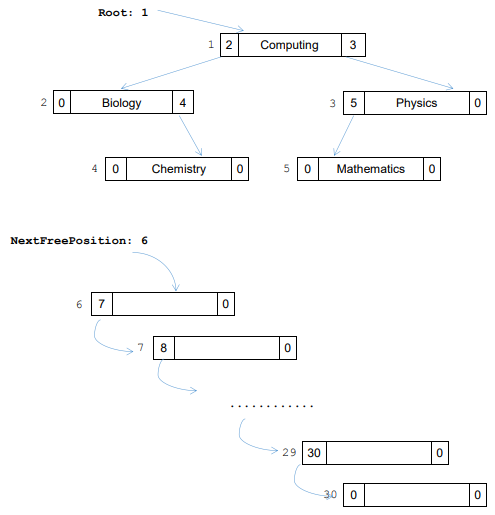
\includegraphics[width=0.5\paperwidth]{C:/Users/Admin/Desktop/Github/question_bank/LyX/static/img/9597-PJC-2016-P1-Q4-1}
\par\end{center}

\subsection*{Task 4.1 }

Write the program code to declare all the required variables and create
the initial linked list which contains all 30 nodes. 

Add statement(s) to initialise the empty tree. 

\subsection*{Evidence 16: }

Your program code for task 4.1. \hfill{}{[}8{]}

The following incomplete pseudocode inserts a data value into the
binary tree structure.

\noindent %
\noindent\begin{minipage}[t]{1\columnwidth}%
\texttt{PROCEDURE InsertBinaryTree(NewItem)}

\texttt{\qquad{}... ... }

\texttt{\qquad{}IF tree is empty }

\texttt{\qquad{}\qquad{}THEN }

\texttt{\qquad{}\qquad{}\qquad{}... ...}

\texttt{\qquad{}ELSE}

\texttt{\qquad{}\qquad{}//traverse the tree to find the insert position }

\texttt{\qquad{}\qquad{}... ... }

\texttt{\qquad{}\qquad{}LastMove = 'X'}

\texttt{\qquad{}\qquad{}REPEAT}

\texttt{\qquad{}\qquad{}\qquad{}PreviousPtr <- CurrentPtr }

\texttt{\qquad{}\qquad{}\qquad{}IF NewItem < CurrentPtr item}

\texttt{\qquad{}\qquad{}\qquad{}\qquad{}THEN }

\texttt{\qquad{}\qquad{}\qquad{}\qquad{}\qquad{}//move left}

\texttt{\qquad{}\qquad{}\qquad{}\qquad{}\qquad{}CurrentPtr <-
CurrentPtr's left pointer}

\texttt{\qquad{}\qquad{}\qquad{}\qquad{}\qquad{}LastMove = 'Left' }

\texttt{\qquad{}\qquad{}\qquad{}\qquad{}ELSE}

\texttt{\qquad{}\qquad{}\qquad{}\qquad{}\qquad{}//move right }

\texttt{\qquad{}\qquad{}\qquad{}\qquad{}\qquad{}CurrentPtr <-
CurrentPtr's right pointer }

\texttt{\qquad{}\qquad{}\qquad{}\qquad{}\qquad{}LastMove = 'Right'}

\texttt{\qquad{}\qquad{}\qquad{}ENDIF }

\texttt{\qquad{}\qquad{}UNTIL CurrentPtr = NULL }

\texttt{\qquad{}ENDIF }

\texttt{\qquad{}IF LastMove = 'Left'}

\texttt{\qquad{}... ... }

\texttt{\qquad{}ELSE IF LastMove = 'Right'}

\texttt{\qquad{}... ...}

\texttt{\qquad{}ENDIF }

\texttt{\qquad{}... ... }

\texttt{END PROCEDURE }%
\end{minipage}

\subsection*{Task 4.2 }

Complete the pseudocode and write a module \texttt{AddSubject} to
add a subject into the binary tree. 

\subsection*{Evidence 17:}

Your \texttt{AddSubject} program code. \hfill{} {[}7{]}

\subsection*{Task 4.3 }

Write a module \texttt{Display} to display the value of \texttt{Root},
the value of \texttt{NextFreePosition} and the contents of \texttt{SubjectTree}
in index order. 

\subsection*{Evidence 18: }

Your \texttt{Display} program code. \hfill{} {[}4{]}

\subsection*{Task 4.4}

Write a module \texttt{BuildTree} to construct a binary tree using
the data provided in the data file \texttt{SUBJECT.TXT}. Read in all
the data from the data file and use the \texttt{AddSubject} module. 

\subsection*{Evidence 19: }

Your \texttt{BuildTree} program code. \hfill{}{[}2{]}

\subsection*{Evidence 20:}

Run your program and produce screenshot of contents of binary tree.
\hfill{} {[}1{]}

Deleting a node from a tree may change the structure of the tree.
To simplify the deletion process, label a node as \textquotedblleft \texttt{deleted}\textquotedblright{}
but \textbf{do not remove the node} from the tree structure. After
that, regenerate the entire tree structure.

\subsection*{Task 4.5 }

Write a module \texttt{LabelDelete} that labels a node as \textquotedblleft \texttt{deleted}\textquotedblright{}
but do not remove the node from the tree structure. 

\subsection*{Evidence 21: }

Your LabelDelete program code. \hfill{}{[}6{]}

\subsection*{Task 4.6}

Write program code to regenerate the entire binary tree.

\subsection*{Evidence 22: }

Your program code to regenerate the binary tree. \hfill{}{[}6{]}

\subsection*{Evidence 23:}

Display a screenshot of the regenerated binary tree after deleting
\textquotedblleft \texttt{Chemistry}\textquotedblright{} and \textquotedblleft \texttt{History}\textquotedblright .
\hfill{} {[}1{]}

{[}SPLIT\_HERE{]}
\item \textbf{{[}PJC/PRELIM/9597/2016/P2/Q1{]} }

The PJC clinic has several doctors. When a patient wants to book an
appointment with a doctor, the patient rings the doctors' receptionist.
The receptionist asks for the following details:
\begin{itemize}
\item patient name 
\item first line of address
\item doctor requested 
\end{itemize}
The receptionist checks the files to ensure that the patient is registered
with the clinic. The receptionist looks to find the requested doctor's
free appointments in the appointments book. The receptionist offers
the patient a day and a time for the appointment. If this is agreed
then the patient's name is written in the space in the appointment
book for that day and time. 

At the beginning of every day, the receptionist types an appointment
list for each of the doctors for that day. The list contains the appointment
times and patients\textquoteright{} names. When the patient arrives
at the doctors' clinic for their appointment, they give their name
to the receptionist. The receptionist informs each doctor as their
patients arrive. 

The clinic has decided to replace this manual system with an on-line
computerised system. 

A \textbf{system developer} is employed to carry out the task. The
first task assigned to the system developer is to write a project
proposal. 
\begin{enumerate}
\item One section of the project proposal is the Problem Statement which
lists the problems in the current system. Write the \textbf{Problem
Statement}. {[}4{]}
\item The system developer has drawn up an initial plan of the work involved: 
\noindent \begin{center}
\begin{tabular}{|c|l|c|}
\hline 
\textbf{Stage} & \textbf{Activity} & \textbf{Weeks}\tabularnewline
\hline 
A & identify requirements & 3\tabularnewline
\hline 
B & produce design & 5\tabularnewline
\hline 
C & write code & 9\tabularnewline
\hline 
D & black box testing & 2\tabularnewline
\hline 
E & acceptance testing & 3\tabularnewline
\hline 
F & prepare documentation & 6\tabularnewline
\hline 
\end{tabular}
\par\end{center}

From this data, a Program Evaluation Review Technique (PERT) chart
is constructed. The stage is between the nodes in circles. 
\begin{center}
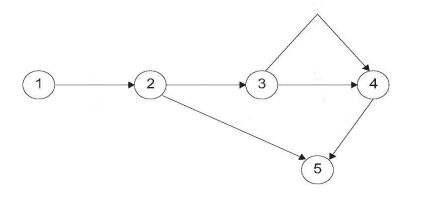
\includegraphics[width=0.5\paperwidth]{C:/Users/Admin/Desktop/Github/question_bank/LyX/static/img/9597-PJC-2016-P2-Q1-1}
\par\end{center}
\begin{enumerate}
\item Complete the PERT chart by writing the stage (A, B, \dots ) and duration
between the nodes. \hfill{}{[}4{]}
\item State the critical path. \hfill{}{[}1{]}
\item State the minimum time in which the project could be completed. \hfill{}{[}1{]}
\item For activity D: 
\begin{enumerate}
\item[(iv.1)]  state the earliest start time. \hfill{}{[}1{]}
\item[(iv.2)]  state the latest finish time. \hfill{}{[}1{]}
\end{enumerate}
\item Two stages start and end at the same nodes. Re-draw the PERT chart
by using an extra dummy stage separating them. Explain the nature
and purpose of a dummy stage. \hfill{}{[}2{]}
\item Explain dependent stages and concurrent stages. For each type of stage
give an example from this chart. \hfill{}{[}4{]}
\item Draw a Gantt chart showing all stages and their dependencies.\hfill{}
{[}4{]}
\end{enumerate}
\item Describe any \textbf{three} key stages (System analysis, System design,
System development, Testing, Implementation of computer system, Documentation,
Maintenance) of the software development life cycle. \hfill{}{[}6{]}
\item Explain why the problem must be defined accurately before the analyst
starts work. \hfill{}{[}2{]}
\item Name two methods the analyst could use to gather information about
the existing manual system. Explain how each method would be used
to gather information about this manual system. \hfill{}{[}4{]}
\item When the receptionist types an appointment for a patient, explain
why the patient name and first line of address need to be entered.
\hfill{}{[}2{]}
\item The following pseudocode algorithm describes one method of finding
an arbitrary patient name in an alphabetically ordered array of \texttt{N}
unique names. 

\noindent\begin{minipage}[t]{1\columnwidth}%
\texttt{SET first to 1 }

\texttt{SET last to N }

\texttt{REPEAT }

\texttt{\qquad{}SET mid to the integer part of (first + last)/2 }

\texttt{\qquad{}IF the mid name precedes the wanted name }

\texttt{\qquad{}\qquad{}THEN SET first to mid + 1 }

\texttt{\qquad{}ELSE }

\texttt{\qquad{}\qquad{}SET last to mid \textendash{} 1 }

\texttt{\qquad{}ENDIF }

\texttt{UNTIL first > last OR mid name is the wanted name }%
\end{minipage}
\begin{enumerate}
\item If 142 patients\textquoteright{} names are stored in the array, and
Natasha is the 44th name, state the elements of the array that are
examined when searching for Natasha.\hfill{} {[}2{]}
\item If a search is made for a name that is not in the array, what is the
largest number of elements that might need to be examined before one
could say that the name is not present? Explain how you arrive at
your answer. \hfill{}{[}2{]}
\end{enumerate}
\item Before releasing the software, it is tested using a variety of strategies.
Describe the following test strategies:
\begin{enumerate}
\item White box testing \hfill{}{[}2{]}
\item Black box testing\hfill{} {[}2{]}
\end{enumerate}
\end{enumerate}
{[}SPLIT\_HERE{]}
\item \textbf{{[}PJC/PRELIM/9597/2016/P2/Q2{]} }

You are the assistant of the system developer. You have been asked
to draw up a plan to provide security within the system you are developing.
Describe measures you can take to ensure 
\begin{enumerate}
\item The reliability and integrity of your data \hfill{}{[}2{]}
\item Physical security\hfill{} {[}2{]}
\item Errors may occur during data transmission. Two methods of checking
for these errors are check sums and parity checks
\begin{enumerate}
\item Explain how a check sum is used to check transmitted data for errors.
\hfill{}{[}2{]}
\item Parity bits can be used to check for errors in transmission and may
also be used to check and self-correct data in blocks. Explain how
parity checks of data blocks can sometimes be used to correct transmission
errors automatically.\hfill{} {[}2{]}
\end{enumerate}
\item Explain the differences between using packet switching and circuit
switching to transmit a message.\hfill{} {[}3{]}
\end{enumerate}
{[}SPLIT\_HERE{]}
\item \textbf{{[}PJC/PRELIM/9597/2016/P2/Q3{]} }

A programmer is going to write part of the new system, using an object-oriented
programming language, which will store details of patients. 

All patients will be identified by their PATIENT\_ID. 

Normal patients will pay cash for their visit but corporate patients
will charge into their company account.

Properties identified type of payments is: 
\begin{itemize}
\item Payment\_type 
\end{itemize}
\begin{enumerate}
\item Draw a diagram that shows how the properties could be distributed
amongst a number of classes. Include in your diagram any inheritance
between classes. Also indicate some of the methods that would be required.
\hfill{}{[}4{]} 
\item In the context of object-oriented programming explain what is meant
by: \hfill{}{[}3{]} 
\begin{enumerate}
\item encapsulation; 
\item inheritance;
\item polymorphism 
\end{enumerate}
\end{enumerate}
{[}SPLIT\_HERE{]}
\item \textbf{{[}PJC/PRELIM/9597/2016/P2/Q4{]} }

An alternative solution for this project is to use cloud computing. 

Discuss briefly the \textbf{three} services that could be used for
the new project. \hfill{}{[}6{]}

{[}SPLIT\_HERE{]}
\item \textbf{{[}PJC/PRELIM/9597/2016/P2/Q5{]} }
\begin{enumerate}
\item The following is a byte stored in a file which contains binary code: 
\noindent \begin{center}
\texttt{10011010 }
\par\end{center}
\begin{enumerate}
\item What is the corresponding denary number? \hfill{} {[}2{]}
\item What is the corresponding hexadecimal number? \hfill{}{[}2{]}
\end{enumerate}
\item An operating system provides a user interface to a computer system. 

Describe two different types of interface that an operating system
provides. \hfill{} {[}4{]}
\item Many modern operating systems support Unicode.
\begin{enumerate}
\item What is Unicode? \hfill{} {[}2{]}
\item What are the advantages of Unicode over ASCII? \hfill{}{[}3{]}
\end{enumerate}
\end{enumerate}
{[}SPLIT\_HERE{]}
\item \textbf{{[}PJC/PRELIM/9597/2016/P2/Q6{]} }

The following shows some data that are stored in a college. 
\noindent \begin{center}
\begin{tabular}{|c|c|c|c|c|c|c|}
\hline 
Student no & Student Name & Programme & Programme Duration (years) & Module No & Module Name & Lecturer\tabularnewline
\hline 
\hline 
13828 & Elvin Gan & P302 & 2 & M165, M121 & Visual Arts, Networking & Fang, Jason\tabularnewline
\hline 
13253 & Goh Seng Lee & P305 & 2 & M121, M110 & Networking, Database & Jason, Kabu\tabularnewline
\hline 
13423 & Yong Kee Le & P502 & 3 & M181, M107, M110 & Music, Accounting, Database & Sunny, Honto, Kabu\tabularnewline
\hline 
13098 & Mahesh Babu & P306 & 4 & M121, M110 & Networking, Database & Jason, Kabu \tabularnewline
\hline 
\end{tabular} 
\par\end{center}

A student is enrolled onto a programme and may take several modules
as part of this programme. A module is only delivered by one lecturer.
\begin{enumerate}
\item These data are in its un-normalised form. Explain the problems associated
with it. \hfill{}{[}2{]}
\item Normalise the data and write them in \textbf{four} tables. \hfill{}{[}6{]}
\item Draw an ER diagram that shows the relationships between these four
tables. \hfill{} {[}2{]}
\end{enumerate}
{[}SPLIT\_HERE{]}
\item \textbf{{[}PJC/PRELIM/9597/2016/P2/Q7{]} }

An online order company charges \$8 for delivery of packages. If the
order value is over \$60, the package is small and the customer has
a promotion code, the delivery is free. If the order value is over
\$60 and the package is small, the delivery charge is \$2. If the
order value is over \$60 and the customer has a promotion code, the
delivery charge is \$2. 
\begin{enumerate}
\item Draw a decision table showing all the possible conditions and actions.
\hfill{}{[}4{]}
\item Simplify your decision table by removing redundancies. \hfill{} {[}2{]}
\end{enumerate}
{[}SPLIT\_HERE{]}
\item \textbf{{[}PJC/PRELIM/9597/2016/P2/Q8{]} }

Consider the following program in pseudocode, which includes a recursive
function that calculates the power of an integer. 

\noindent %
\noindent\begin{minipage}[t]{1\columnwidth}%
\texttt{010 PROGRAM }

\texttt{020}

\texttt{030 FUNCTION Power(Base: INTEGER, Exponent: INTEGER) RETURN }

\texttt{040 INTEGER }

\texttt{050 \qquad{}IF Exponent = 0 }

\texttt{060 \qquad{}\qquad{}THEN }

\texttt{070 \qquad{}\qquad{}\qquad{}Result <- 1}

\texttt{080 \qquad{}\qquad{}ELSE }

\texttt{090 \qquad{}\qquad{}\qquad{}Result <- Base {*} Power(Base,
Exponent \textendash{} 1)}

\texttt{100 \qquad{}ENDIF }

\texttt{110 \qquad{}RETURN Result }

\texttt{120 ENDFUNCTION}

\texttt{130 }

\texttt{140~// main program}

\texttt{150 DECLARE Answer: INTEGER, Base: INTEGER, Exponent: INTEGER }

\texttt{160 INPUT Base }

\texttt{170 INPUT Exponent }

\texttt{180 Answer <- Power(Base, Exponent) }

\texttt{~~~~OUTPUT Answer }%
\end{minipage}
\begin{enumerate}
\item Trace the execution of the function call \texttt{Power(2,3)}, showing
for each re-entry into the \texttt{Power} function, the values passed
to the function and the results returned.\hfill{} {[}3{]}
\end{enumerate}
The program is executed, starting from line 140.
\begin{enumerate}
\item[(b)]  Explain how the stack content changes during the execution of the
program, with input of 2 for \texttt{Base} (line 150), and 3 for \texttt{Exponent}
(line 160).\hfill{} {[}4{]}
\item[(c)]  Write a pseudocode for a non-recursive version of the \texttt{Power}
function. \hfill{}{[}3{]}
\item[(d)]  State one reason why a non-recursive \texttt{Power} function may
be preferred to a recursive one. \hfill{}{[}1{]}
\end{enumerate}
{[}SPLIT\_HERE{]}
\item \textbf{{[}PJC/PRELIM/9597/2016/P2/Q9{]} }

A linked list is stored in an array of records. One record represents
a node and consists of the data and a pointer. 

The diagram shows an implementation of an \textbf{ordered linked list}
before any data is inserted into it. NULL is represented by a value
of 0. 
\noindent \begin{center}
\begin{tabular}{cccc|c|c|}
 &  &  & \multicolumn{1}{c}{} & \multicolumn{2}{c}{\texttt{List}}\tabularnewline
 &  &  & \multicolumn{1}{c}{} & \multicolumn{1}{c}{\texttt{Data}} & \multicolumn{1}{c}{\texttt{Pointer}}\tabularnewline
\cline{5-6} \cline{6-6} 
 &  &  & {[}1{]} &  & 2\tabularnewline
\cline{2-2} \cline{5-6} \cline{6-6} 
\multicolumn{1}{c|}{Start} & \multicolumn{1}{c|}{0} &  & {[}2{]} &  & 3\tabularnewline
\cline{2-2} \cline{5-6} \cline{6-6} 
 &  &  & {[}3{]} &  & 4\tabularnewline
\cline{2-2} \cline{5-6} \cline{6-6} 
\multicolumn{1}{c|}{NextFree} & \multicolumn{1}{c|}{1} &  & {[}4{]} &  & 5\tabularnewline
\cline{2-2} \cline{5-6} \cline{6-6} 
 &  &  & {[}5{]} &  & 6\tabularnewline
\cline{5-6} \cline{6-6} 
 &  &  & {[}6{]} &  & 7\tabularnewline
\cline{5-6} \cline{6-6} 
 &  &  & {[}7{]} &  & 0\tabularnewline
\cline{5-6} \cline{6-6} 
\end{tabular}
\par\end{center}
\begin{enumerate}
\item Show the state of the \textbf{ordered linked list} after \textbf{three}
data items have been added to it in the given order: \emph{Paris},
\emph{Tokyo}, \emph{Santiago}.\hfill{} {[}2{]}
\item Write the algorithm for the procedure to insert a new node into an
ordered linked list. Use the identifiers above and include suitable
annotations.\hfill{} {[}7{]}
\item Describe how a stack can be implemented as a linked list. \hfill{}{[}3{]}
\end{enumerate}
{[}SPLIT\_HERE{]}
\end{enumerate}

\end{document}
